\chapter{Algebraic quantum formalism}
\label{s:AlgQM}
\section{Introduction}
In this formulation, quantum mechanics is constructed from the classical concepts of observables and states, assuming  that observables are not  commuting quantities anymore 
but still form an algebra, and using the concepts of causality and reversibility. Of course such ideas go back to the matrix mechanics of Heisenberg, but the precise formulation relies on the mathematical theory of operator algebras, initiated by F. J. Murray and J. von Neumann 
\index{von Neumann J.}
in the end of the thirties (one motivation of J. von Neumann was precisely to understand quantum mechanics). It was developped by Segal (Segal 47), and then notably by Wightman, Haag, Kastler, Ruelle, etc.

The standard and excellent reference on the algebraic and axiomatic approaches to quantum field theory is the book by R. Haag, Local Quantum Physics,  especially the second edition (1996) \cite{Haag96}. 
Another older reference is the book by N. N. Bogoliubov; A. A. Logunov, A.I. Oksak and  I.T. Todorov (1975, 1990) \cite{Bogo-Todo90}. 
Another useful reference is the famous book by R. F. Streater and A. S. Wightman (1964, 1989) \cite{StreaterWightmanBook} .


Standard references on operator algebras in the mathematical litterature are the books by J. Dixmier (1981, 1982)  \cite{Dixmier:1969vn}, Sakai (1971) \cite{Sakai71}, P. de la Harpe and V. Jones (1995) \cite{delaHarpeJones95}. References more oriented towards the (mathematical) physics community are Bratteli and Robinson(1979) \cite{BratteliRobinson2002}, A. Connes (1994) \cite{Connes94} and A. Connes and M. Marcolli \cite{ConnesMarcolli07}.
 I shall need also some results on real $\mathrm{C}^*$-algebras and the only good reference I am aware of is Goodearl (1982) \cite{Goodearl82}.
 
 I shall give here a very brief and crude presentation of the algebraic formulation of quantum theory. 
 It will stay at a very heuristic level, with no claim of precision or of mathematical rigor.
 However the starting point will be a bit different from the usual presentation, and was presented in \cite{PhysRevLett.107.180401}. 
 I shall start from the general concepts of observables and states, and derive why \emph{abstract real C$^*$-algebras} are the natural framework to formulate quantum theories. 
 Then I shall explain which mathematical results ensure that the theory can always be represented by algebras of operators on Hilbert spaces. 
 Finally I shall explain why locality and separability enforce the use of complex algebras and of complex Hilbert spaces.




{
\section{The algebra of observables}
}

\subsection{The mathematical  principles}
\label{AxiomsAlg}
A quantum system is described by its observables, its states and a causal involution acting on the observables and enforcing constraints on the states. Let us first give the axioms and motivate them later on.

\subsubsection{Observables}
 \index{Observable}\index{Real algebra}\index{Associatice algebra}\index{Unital algebra}
 The physical observables of the system generate  a \emph{real associative unital algebra $\mathcal{A}$} (whose elements will still be denoted ``observables'' ) .
 $\mathcal{A}$ is a linear vector space
  \begin{equation*}
\label{ }
\mathbf{a},\,\mathbf{b}\in \mathcal{A}\quad \lambda,\, \mu\in\mathbb{R}
\qquad
\lambda \mathbf{a} +\mu \mathbf{b} \in A 
\end{equation*}
\index{Associativity}\index{Distributivity}
with an associative product (distributive w.r.t the addition)
 \begin{equation}
\label{algebra}
\mathbf{a},\,\mathbf{b},\,\mathbf{c}\in \mathcal{A}
\qquad\mathbf{ab}\in A
\qquad
(\mathbf{ab})\mathbf{c}=\mathbf{a}(\mathbf{bc})
\end{equation}
and an unity
\begin{equation}
\label{ }
\mathbf{1 a}=\mathbf{a 1}=\mathbf{a}\ ,\ \ \forall \mathbf{a}\in\mathcal{A}
\end{equation}
We shall precise later what are ``physical observables''.


\subsubsection{The $^*$-conjugation}
\index{Conjugation}\index{Involution}\index{Anti-automorphism}
There is an involution $^\star$ on $\mathcal{A}$ (denoted conjugation). It is an anti-automorphism whose square is the identity. This means that
  \begin{equation*}
\label{ }
(\lambda \mathbf{a}+\mu \mathbf{b})^\star = \lambda \mathbf{a}^\star  + \mu \mathbf{b}^\star  
\end{equation*}
 \begin{equation}
\label{involution}
{(\mathbf{a}^*)}^*=\mathbf{a}
\qquad (\mathbf{ab})^\star =\mathbf{b}^\star  \mathbf{a}^\star 
\end{equation}

\subsubsection{States}
\index{State}\index{Expectation value}
   Each $\varphi$ associates to an observable $\mathbf{a}$ its expectation value $\varphi(\mathbf{a})\in\mathbb{R}$ in the state $\varphi$.
The states satisfy
  \begin{equation*}
\label{ }
\varphi(\lambda \mathbf{a} +\mu \mathbf{b})=\lambda \varphi(\mathbf{a}) +\mu \varphi(\mathbf{b})
\end{equation*}
  \begin{equation}
\label{defsta}
\varphi(\mathbf{a}^\star )=\varphi(\mathbf{a}) \qquad \varphi(\mathbf{1})=1 \qquad \varphi(\mathbf{a}^\star \mathbf{a})\ge 0
\end{equation}
The set of states is denoted $\mathcal{E}$. It is natural to assume that it allows to discriminate between observables, i.e.
\begin{equation}
\label{ }
\forall \ \mathbf{a}\neq\mathbf{b}\in\mathcal{A} \ (\text{and}\ \neq \mathbf{0}), \exists\  \varphi\in\mathcal{E}\ \text{such that}\ \varphi(\mathbf{a})\neq\varphi(\mathbf{b})
\end{equation}

I do not discuss the concepts of time and dynamics at that stage. This will be done later. I first discuss the relation between these ``axioms'' and the physical concepts of causality, reversibility and probabilities.

\subsection{Physical discussion}
\subsubsection{Observables and causality}
\index{Causality}
{
In quantum physics, the concept of physical observable corresponds both to an operation on the system (measurement) and to the response on the system (result on the measure), but I shall not elaborate further. 
We already discussed why in classical physics observables form a real commutative algebra. The removal of the commutativity assumption is the simplest modification imaginable compatible with the uncertainty principle (Heisenberg 1925).

Keeping the mathematical structure of an associative but non commutative algebra reflects the assumption that there is still some concept of \og causal ordering\fg\   
 between observables (not necessarily physical), in a formal but  loose sense. 
Indeed the multiplication and its associativity means that we can \og combine\fg{} successive observables, e.g. $\mathbf{ab}\simeq (\mathbf{b}$ then $\mathbf{a}$), in a linear process such that (($\mathbf{c}$ then $\mathbf{b}$) then $\mathbf{a}) \simeq (\mathbf{c}$ then ($\mathbf{b}$ then $\mathbf{a}$)). This ``combination'' is different from the concept of ``successive measurement".
\index{Non commutative algebra}

Without commutativity the existence of an addition law is already a non trivial fact, it means that we can \og combine\fg{} two non compatible observations into a new one whose mean value is always the sum of the first two mean values.

Both addition and mutiplication of observables are in fact more natural in the context of relativistic theories, via the analyticity properties of correlation functions and the short time and short distance expansions.
 
 \subsubsection{The $^*$-conjugation and reversibility}
 \index{Conjugation}\index{Irreversibility}
 The existence of the involution $^*$ (or conjugation) is the second and very important feature of quantum physics. It implies that although the observables do not commute, there is no favored arrow of time (or causal ordering) in the formulation of a physical theory, in other word this is reversibility. To any causal description of a system in term of a set of  observables $\{\mathbf{a},\,\mathbf{b},\,\ldots\}$ corresponds an equivalent \og anti-causal\fg{} description it terms of  conjugate observables $\{\mathbf{a}^*,\,\mathbf{b}^*,\,\ldots\}$. Although there is no precise concept of time or dynamics yet, the involution $^*$ must not be confused with the time reversal operator $\mathbf{T}$ (which may or may not be a symmetry of the dynamics).
 
\subsubsection{States, mesurements and probabilities}
\index{State}\index{Measurement}\index{Probabilities}
The states $\varphi$ are the simple generalisation of the classical concept of statistic (or probabilistic) states describing our knowledge of a system through the expectation value of the outcome of measurements for each possible observables. At that stage we do not assume anything about whether there are states such that all the values of the observables can be determined or not. Thus a state can be viewed also as the characterization of all the information which can be extracted from a system through a measurement process (this is the point of view often taken in quantum information theory).
We do not consider how states are prepared, nor how the measurements are performed (this is the object of the subpart of quantum theory known as the theory of quantum measurement) and just look at the consistency requirements on the outcome of measurements.

The \og expectation value\fg{} $\varphi(\mathbf{a})$ of an observable $\mathbf{a}$ can be considered as well as given by the average of the outcome of measurements $\mathbf{a}$  over many realisations of the system in the same state (frequentist view) or as the sum over the possible outcomes $a_i$ times the plausibility for the outcomes  in a given state (Bayesian view).
\index{Measurement}\index{Frequentist probabilities}\index{Bayesian probabilities}
In fact both point of views have to be considered, and are somehow unified, in the quantum formalism.


The linearity of the $\varphi$'s follows from (or is equivalent to) the assumptions that the observables form a linear vector space on $\mathbb{R}$.

The very important condition $$\varphi(\mathbf{a}^*)=\varphi(\mathbf{a})$$
 for any $\mathbf{a}$ follows from the assumption of reversibility. If this were not the case, there would be observables which would allow to favor one causal ordering, irrespective of the dynamics and of the states of the system.
 \index{Reversibility}

The positivity condition $\varphi(\mathbf{a}^*\mathbf{a})\ge 0$ ensures that the states have a probabilistic interpretation, so that on any state the expectation value of a positive observable is positive, and that there are no  negative probabilities, in other word it will ensure unitarity.
It is the simplest consistent positivity condition compatible with reversibility, and in fact the only possible without assuming more structure on the observables. 
Of course the condition $\varphi(\mathbf{1})=1$ is the normalisation condition for probabilities.
\index{Positivity}

\subsection{Physical observables and pure states}
Three important concepts follow from these principles.
\subsubsection{Physical (symmetric) observables:}
An observable $\mathbf{a}\in\mathcal{A}$ is symmetric (self adjoint, or self conjugate) if $\mathbf{a}^*=\mathbf{a}$.
Symmetric observables correspond to the physical observables, which are actually measurable. 
Observable such that $\mathbf{a}^*=-\mathbf{a}$ are skew-symmetric (anti-symmetric or anti conjugate). They do not correspond to physical observables but must be included in order to have a consistent algebraic formalism.
\index{Physical observable}

\subsubsection{Pure states:}
The set of states $\mathcal{E}$ is a convex subset of the set of real linear forms on $\mathcal{A}$ (the dual of  $\mathcal{A}$). Indeed if $\varphi_1$ et $\varphi_2$ are two states and $0\le x\le 1$, $\varphi=x \varphi_1+(1-x) \varphi_2$ is also a state.
This corresponds to the fact that any statistical mixture of two statistical mixtures is a statistical mixture.
Then the extremal points in  $\mathcal{E}$, i.e. the states which cannot be written as a statistical mixture of two differents states in $\mathcal{E}$, are called the pure states. Non pure states are called mixed states. If a system is in a pure state one cannot get more information from this system than what we have already.
\index{Pure state}

\subsubsection{Bounded observables}
We just need to impose two additional technical and natural assumptions:
(i)  for any observable $\mathbf{a}\neq 0$, there is a state $\varphi$ such that $\varphi(\mathbf{a}^*\mathbf{a})>0$, if this is not the case, the observable $\mathbf{a}$ is indistinguishable from the observable $0$ (which is always false); 
(ii) $\sup_{\varphi\in\mathcal{E}} \varphi(\mathbf{a}^*\mathbf{a})<\infty$, i.e. we restrict $\mathcal{A}$ to the algebra of bounded observables, this will be enough to characterize the system.
\index{Bounded observable}


\section{The C$^*$-algebra of observables}
\label{RCstarAlg}


The involution $^*$ et the existence of the states $\varphi\in \mathcal{E}$ on $\mathcal{A}$  strongly constrain  the structure of the algebra of observables and of its representations. 
Indeed this allows to associate to $\mathcal{A}$ a unique norm $\| \cdot \|$  with some specific properties. This norm makes $\mathcal{A}$ a $\mathrm{C}^*$-algebra, and more precisely a real abstract $\mathrm{C}^*$-algebra.
\index{C$^*$-algebra}
\index{Abstract C$^*$-algebra}
This structure  justifies the standard representation of quantum mechanics where pure states are elements of an Hilbert space and physical observables are  self-adjoint operators.

\subsection{The norm on observables, $\mathcal{A}$ is a Banach algebra}
\index{Norm}
Let us consider the  function $\mathbf{a}\to ||\mathbf{a}||$  from $\mathcal{A}\to\mathbb{R}^+$ defined by
\begin{equation}
\label{normstate}
||\mathbf{a}||^2=\sup_{\mathrm{states}\,\varphi\in\mathcal{E}}\varphi(\mathbf{a}^\star \mathbf{a})
\end{equation}
We have assumed that 
$||\mathbf{a}||<\infty$, $\forall a\in\mathcal{A}$ and that $||\mathbf{a}||=0\iff\mathbf{a}=0$ (this is equivalent to $\mathbf{a}\neq 0\implies\exists \varphi\in\mathcal{E}$ such that $\varphi(\mathbf{a^*a})\neq 0$). It is easy to show that  $||\cdot ||$ is a norm on $\mathcal{A}$, such that
\begin{equation}
\label{ }
||\lambda \mathbf{a}||=|\lambda|\,||\mathbf{a}||
\qquad
||\mathbf{a}+\mathbf{b}||\le�||\mathbf{a}||+||\mathbf{b}||
\qquad
||\mathbf{ab}||\le ||\mathbf{a}||\,||\mathbf{b}||
\end{equation}
If  $\mathcal{A}$ is not closed for this norm, we can take  its completion  $\overline{\mathcal{A}}$.  The algebra of observables is therefore a real Banach algebra.
\index{Banach algebra}


\paragraph{Derivation:}\ 

The first identity comes from the definition and the linearity of states.

Taking $\mathbf{c}=x\mathbf{a}+(1-x)\mathbf{b}$ and using the positivity of $\varphi(c^*c)\ge 0$ for any $x\in\mathbb{R}$ we obtain Schwartz inequality
$\varphi(a^*b)^2=\varphi(a^*b)\varphi(b^*a)\le \varphi(a^*a)\varphi(b^*b)$, $\forall\, a,\,b\in\mathbf{A}$. This implies the second inequality.
\index{Positivity}
\index{Schwartz inequality}

The third inequality comes from the fact that if
$\varphi \in\mathcal{E}$ and $b\in\mathcal{A}$ are such that $\varphi(b^*b)>0$, then $\varphi_b$ defined by
$\varphi_b(a)={\varphi(b^*ab)\over \varphi(b^*b)}$
is also a state for $\mathcal{A}$.
Then
$
||ab||^2= \sup_\varphi \varphi(b^*a^*ab)=\sup_\varphi \varphi_b(a^*a) \varphi(b^*b)\le \sup_g g(a^*a)\ \sup_\varphi \varphi(b^*b)=|| a||^2\, ||b||^2
$.


\subsection{The observables form a real $\mathrm{C}^*$-algebra}
Moreover the norm satisfies the two non-trivial properties.
\begin{equation}
\label{C*cond}
||\mathbf{a}^* \mathbf{a}||=||\mathbf{a}||^2=|| \mathbf{a}^*||^2
\end{equation}
and
\begin{equation}
\label{invcond}
\mathbf{1}+\mathbf{a}^*\mathbf{a}\quad\text{is invertible}\quad\forall\, \mathbf{a}\in \mathcal{A}
\end{equation}
These two properties are equivalent to state that  $\mathcal{A}$ is a real C$^*$-algebra.
\index{Real C$^*$-algebra}
\footnote{The  first condition on the norm and the involution \ref{C*cond} is sometimes called the C$^*$ condition. The \og C\fg{} letter in the denomination C$^*$-algebra originally comes from term  \og closed\fg{}, the closure condition specific to subalgebras of the algebra of bounded operators on a Hilbert space which defines also C$^*$-algebras. 
The second condition \ref{invcond} is specific to real algebras.}.
For a definition of real C$^*$-algebras and the properties used below see the book by Goodearl \cite{Goodearl82}. 



\paragraph{Derivation:}\ 

One has $||a^*a||\le ||a||\,||a^*||$.
Schwartz inequality implies that  
$\varphi(a^*a)^2\le \varphi\left( (a^*a)^2\right) \varphi(1)$, hence $||a||^2\le ||a^*a||$. This implies (\ref{C*cond}).

To obtain (\ref{invcond}), notice that if  $1+a^*a$ is not inversible, there is a $b\neq 0$ such that $(1+a^*a)b=0$, hence $b^*b+(ab)^*(ab)=0$. Since there is a state $\varphi$ such that $\varphi(b^*b)\neq 0$, either $\varphi(b^*b)<0$ or $\varphi((ab)^*(ab)<0$, this contradicts the positivity of states.


\medskip

The full consequences will be discussed in next subsection. Before that we can introduce already the concept of spectrum of an observable.

\subsection{Spectrum of observables and results of measurements}
Here I discuss in a slightly more precise way the relationship between the spectrum of observables and results of measurements.
The spectrum 
\footnote{The exact definition is slightly different for a general real Banach algebra.}
 of an element $\mathbf{a}\in\mathcal{A}$ is defined as  $$\mathrm{Sp}^{\scriptscriptstyle{\mathbb{C}}}(\mathbf{a})=\{z\in\mathbb{C}:\ (z-\mathbf{a})\ \text{not inversible in}\ \mathcal{A}_{\mathbb{C}}\ \text{the complexified of}\ \mathcal{A}\}\ \ .$$
The spectral radius of $\mathbf{a}$ is defined as
\index{Spectrum}\index{Spectral radius}
$$
r^{\scriptscriptstyle{\mathbb{C}}}(\mathbf{a})=\sup( |z|;\ z\in
\mathrm{Sp}^{\scriptscriptstyle{\mathbb{C}}}(\mathbf{a}))
$$
For a real C$^*$-algebra it is known that the norm  $||\cdot||$ defined by \ref{normstate} is
$$ ||a||^2=r^{\scriptscriptstyle{\mathbb{C}}}(\mathbf{a}^*\mathbf{a})$$
that the spectrum of  any physical observable (symetric) is real
$$
\mathbf{a}=\mathbf{a}^*\ \implies\ \mathrm{Sp}^{\scriptscriptstyle{\mathbb{C}}}(\mathbf{a})\subset\mathbb{R}
$$
and that for any $\mathbf{a}$, the product  $\mathbf{a^*a}$ is a symmetric positive element of $\mathcal{A}$, i.e. its spectrum is real and positive
$$
\mathrm{Sp}^{\scriptscriptstyle{\mathbb{C}}}(\mathbf{a^*a})\subset\mathbb{R}^+
$$
Finally, for any (continuous) real function $F$ $\mathbb{R}\to\mathbb{R}$ and any $\mathbf{a}\in\mathcal{A}$ one can define the observable $F(\mathbf{a})$. Now consider a physical observable $\mathbf{a}$.
Physically, measuring $F(\mathbf{a})$ amounts to measure $\mathbf{a}$ and when we get the real number $A$ as a result, return $F(A$) as a result of the measure of $F(\mathbf{a})$ (this is fully consistent with the algebraic definition of $F(\mathbf{a})$ since $F(\mathbf{a})$ commutes with $\mathbf{a}$).
Then is can be shown easily that the spectrum of $F(\mathbf{a})$ is the image by $F$ of the spectrum of $\mathbf{a}$, i.e. 
$$\mathrm{Sp}^{\scriptscriptstyle{\mathbb{C}}}(F(\mathbf{a}))=F(\mathrm{Sp}^{\scriptscriptstyle{\mathbb{C}}}(\mathbf{a}))$$
In particular, assuming that the spectrum is a discrete set of points, let us  choose for $F$ the function 
$$F[\mathbf{a}]=1/(z\mathbf{1}-\mathbf{a})$$
For any state $\varphi$, the expectation value of this observable on the state $\varphi$ is 
$$E_\varphi(z)=  \varphi(1/(z\mathbf{1}-\mathbf{a})$$ and is an analytic function of $z$ away from the points of the spectrum $\mathrm{Sp}^{\scriptscriptstyle{\mathbb{C}}}(\mathbf{a}))$. (Assuming that the singularity at each $z_p$ is  a single pole) the residue of $E_\varphi(z)$ at $z_p$ is nothing but
\begin{align}
\label{Probzp}
    Res_{z_p}E_\varphi &  =\ \varphi(\delta(\mathbf{a}-z_p\mathbf{1}))  \nonumber \\
    &=\   \text{probabiliy to obtain}\ z_p\ \text{when measuring}\  \mathbf{a}\  \text{on the state}\  \varphi  
\end{align}
with $\delta(z)$ the Dirac distribution.
\index{Dirac distribution}\index{Physical observable}\index{Measurement}\index{Output of a measurement}

This implies that for any physical observable $\mathbf{a}$, its spectrum is the set of all the possible real numbers $z_p$ returned by a measurement of $\mathbf{a}$. This is one of the most important axioms of the standard formulation of quantum mechanics, and we see that it is a consequence of the axioms in this formulation. Of course the probability to get a given value $z_p$ (an element of the spectrum) depends on the state $f$ of the system, and it is given by \ref{Probzp} which is nothing but  some kind of Born rule for the abstract definiton of states.
\index{Born rule}

\subsection{Complex C$^*$-algebras}
The theory of operator algebras (C$^*$-algebras and W$^*$-algebras) and their applications (almost) exclusively deal with complex algebras, i.e. algebras over $\mathbb{C}$. 
In the case of quantum physics we shall see a bit later why  quantum (field) theories must be represented by complex C$^*$-algebras. I give here some definitions.
\index{C$^*$-algebra}\index{Abstract C$^*$-algebra}\index{Complex C$^*$-algebra}
\index{Associative algebra}\index{Involution}

Abstract complex $C^*$-algebras and complex states $\phi$ are defined as in \ref{AxiomsAlg}.
A complex C$^*$-algebra  $\mathfrak{A}$ is a complex associative involutive algebra.
The involution is now anti-linear
\index{Antilinear application}
$$(\lambda \mathbf{a}+\mu \mathbf{b})^\star = \bar\lambda \mathbf{a}^\star  + \bar\mu \mathbf{b}^\star
\qquad \lambda,\,\mu\in\mathbb{C}$$ 
$\bar z $ denotes the complex conjugate of $z$.
$\mathfrak{A}$ has a norm $\mathbf{a}\to ||\mathbf{a}||$ which still satisfy the C$^*$ condition  \ref{C*cond}, 
\begin{equation}
\label{C*condC}
||\mathbf{a}^* \mathbf{a}||=||\mathbf{a}||^2=|| \mathbf{a}^*||^2
\end{equation}
and it is closed under this norm.
The condition \ref{invcond} is not necessary any more (it follows from \ref{C*condC} for complex algebras).

The states are defined now as the complex linear forms $\phi$ on $\mathfrak{A}$ which satisfy
\begin{equation}
\label{ }
\phi(\mathbf{a}^*)=\overline{\phi(\mathbf{a})}
\qquad
\phi(\mathbf{1})=1
\qquad
\phi(\mathbf{a}^*\mathbf{a})\ge 0
\end{equation}
Any complex C$^*$-algebra $\mathfrak{A}$ can be considered as a real C$^*$-algebra $\mathcal{A}_{\mathbb{R}}$ (by considering $\imath=\sqrt{-1}$ as an element $\mathbf{i}$ of the center of $\mathcal{A}_{\mathbb{R}}$) but the reverse is not true in general. 
\index{Center of an algebra}

However if a real algebra $\mathcal{A}_{\mathbb{R}}$ has an element (denoted $\mathbf{i}$) in its center $\mathcal{C}$ that is isomorphic to $\sqrt{-1}$, i.e. $\mathbf{I}$ is such that
\begin{equation}
\label{ }
\mathbf{i}=-\mathbf{i}\ ,\  \mathbf{i}^2=-\mathbf{1}\ ,\ \ \mathbf{i a}=\mathbf{a i}\ \ \forall\ \mathbf{a}\in \mathcal{H}_{\mathbb{R}}
\end{equation}
then the algebra $\mathcal{A}_{\mathbb{R}}$ is isomorphic to a complex algebra $\mathcal{A}_{\mathbb{C}}=\mathfrak{A}$. One identifies $x\mathbf{1}+y\mathbf{i}$ with the complex scalar $z=x+\imath y$.
The conjugation $^*$ (linear on $\mathcal{A}_{\mathbb{R}}$) is now anti-linear on $\mathcal{A}_{\mathbb{C}}$.
One can associate to each  $\mathbf{a}\in\mathcal{A}_{\mathbb{R}}$ its real and imaginary part
\begin{equation}
\label{ }
\Re(\mathbf{a})={\mathbf{a}+\mathbf{a}^*\over 2}
\ ,\ \ 
\Im(\mathbf{a})=\mathbf{i}{\mathbf{a}^*-\mathbf{a}\over 2}
\end{equation}
and write in $\mathcal{A}_{\mathbb{C}}$
\begin{equation}
\label{ }
\mathbf{a}=\Re(\mathbf{a})+\imath\ \Im(\mathbf{a})
\end{equation}
To any real state (and in fact any real linear form) $\varphi_{\mathbb{R}}$ on $\mathcal{H}_{\mathbb{R}}$ one associates the complex state (the complex linear form) $\phi_{\mathbb{C}}$ on $\mathcal{A}_{\mathbb{C}}$ defined as
\begin{equation}
\label{ }
\phi_{\mathbb{C}}(\mathbf{a})=\varphi_{\mathbb{R}}(\Re(\mathbf{a}))+\imath\, \varphi_{\mathbb{R}}(\Im(\mathbf{a}))
\end{equation}
It has the expected properties for a complex state on the complex algebra $\mathfrak{A}$.


\section{The GNS construction, operators and Hilbert spaces}
General theorems show that abstract C$^*$-algebras can always be represented as algebra of operators on some Hilbert space. This is the main reason why pure states are always represented by vectors in a Hilbert space and observables as operators. Let us briefly consider how this works.


\subsection{Finite dimensional algebra of observables}
Let us first consider the case of finite dimensional algebras, which corresponds to quantum system with a finite number of independent quantum states.
This is the case considered in general in quantum information theory.
\index{Finite dimensional algebra}

If $\mathcal{A}$ is a finite dimensional real algebra, one can show by purely algebraic methods that $\mathcal{A}$ is a direct sum of matrix algebras over $\mathbb{R}$, $\mathbb{C}$ or $\mathbb{H}$ (the quaternions).
See \cite{Goodearl82} for details. The idea is to show that the C$^*$-algebra conditions  implies that the real algebra $\mathcal{A}$ is semi-simple (it cannot have a nilpotent two-sided ideal) and to use the Artin-Wedderburn theorem. 
\index{Artin-Wedderburn theorem}
\index{Quaternion}
One can even relax the positivity condition $\varphi(\mathbf{a}^*\mathbf{a})\ge 0$ for any $\mathbf{a}$ to the condition $\varphi(\mathbf{a}^2)\ge 0$ for physical observables $\mathbf{a}=\mathbf{a}^*$, which is physically somewhat more satisfactory (F. David unpublished, probably known in the math litterature...).
Thus the algebra is of the form
\begin{equation}
\label{ }
\mathcal{A}=\bigoplus_{i} M_{n_i}(K_i)\qquad K_i=\mathbb{R},\ \mathbb{C},\ \mathbb{H}
\end{equation}
The index $i$ label the components of the center of the algebra.
Any observable reads
$$
\mathbf{a}=\oplus_i \mathbf{a}_i\ ,\ \ \mathbf{a}_i  \in\mathcal{A}_i=M_{n_i}(K_i) 
$$
The multiplication corresponds to the standard matrix multiplication and the involution $^*$ to the standard conjugation (transposition, transposition+complex conjugation and transposition+conjugation respectively for real, complex and quaternionic matrices). 
One thus recovers the familiar matrix ensembles of random matrix theory.
\index{Random matrix}

Any state $\omega$ can be written as
\index{State}
$$\omega(\mathbf{a})=\sum_i p_i\,\tr(\boldsymbol{\rho}_i\mathbf{a}_i)  
\qquad p_i\ge 0,\quad \sum_i p_i=1
$$
and the $\boldsymbol{\rho}_i$'s some symmetric positive normalised matrices in each $\mathcal{A}_i$
$$
\boldsymbol{\rho}_i\in\mathcal{A}_i=M_{n_i}(K_i) \ ,\quad \boldsymbol{\rho}_i= \boldsymbol{\rho}_i^*\ ,\quad \tr(\boldsymbol{\rho}_i)=1\ ,\quad \boldsymbol{\rho}_i\ge 0
$$
The algebra of observables is indeed a subalgebra of the algebra of operators on a finite dimensional real Hilbert space $\mathcal{H}=\bigoplus_i K_i^{n_i}$ ($\mathbb{C}$ and $\mathbb{H}$ being considered as 2 dimensional and 4 dimensional real vector spaces respectively).
But it is not necessarily the whole algebra $\mathcal{L}(\mathcal{H})$.
The system corresponds to a  disjoint collection of standard quantum systems described by their Hilbert space $\mathcal{H}_i=K_i^{n_i}$ and their algebra of observables $\mathcal{A}_i$. 
This decomposition is (with a bit of abuse of language) a decomposition into superselection sectors\footnote{For many authors the term of superselection sectors is reserved to infinite dimensional algebras which do have inequivalent representations.}.
The  $\boldsymbol{\rho}_i$ are the quantum density matrices corresponding to the state. The $p_i$'s correspond to the classical probability to be in a given sector, i.e. in a state described by $(\mathcal{A}_i,\mathcal{H}_i)$. 

A pure state is (the projection onto a) single vector $|\psi_i\rangle$ in a single sector $\mathcal{H}_i$.
\index{Pure state}
Linear superpositions of pure states in different sectors $|\psi\rangle=\sum_i c_i |\psi_i\rangle$ do not make sense, since they do not belong to the representation of $\mathcal{A}$.
No observable $\mathbf{a}$ in $\mathcal{A}$ allows to discriminate between the seemingly-pure-state $|\psi\rangle\langle\psi|$ and the mixed state
$\sum_i |c_i|^2 |\psi_i\rangle\langle \psi_i|$.
Thus the different sectors can be viewed as describing completely independent systems with no quantum correlations, in other word really parallel universes with no possible interaction or communication between them.
\index{Superselection sector}

\subsection{Infinite dimensional real algebra of observables}
\index{Infinite dimensional algebra}
This result generalizes to the case of infinite dimensional real C$^*$-algebras, but it is much more difficult to prove, analysis and topology enter in the game and the fact that the algebra is closed under the norm is crucial (for a physicist this is a natural requirement).

\paragraph{Theorem (Ingelstam NN \cite{Ingelstam64,Goodearl82}):} For any real C$^*$-algebra, there exists a real Hilbert space $\mathcal{H}$ such that $\mathcal{A}$ is isomorphic to a real symmetric closed real sub-algebra of the algebra $B(\mathcal{H})$ of bounded operators on $\mathcal{H}$.
\index{Bounded operator}

\paragraph{}Now any real algebra of symmetric operators on a real Hilbert space $\mathcal{H}$ may be extended (by standard complexification) into a complex algebra of self-adjoint operator on a Hilbert space $\mathcal{H}_{\mathbb{C}}$ on $\mathbb{C}$ and thus one can reduce the study of real algebra to the study of complex algebra. In particular the theory of representations of real C$^*$-algebra is not really richer than that of complex C$^*$-algebra and mathematicians usuallyI  considers only the later case.

I will discuss later why in quantum physics one should restrict oneself also to complex algebras.
But note that in physics real (and quaternionic) algebra of observables do appear as the subalgebra of observables of some system described by a complex Hilbert space, subjected to some additional symmetry constraint (time reversal invariance $\mathbf{T}$ for real algebra, time reversal and an additional SU(2) invariance for quaternionic algebras). 


\subsection{The complex case, the GNS construction}

\index{Complex C$^*$-algebra}\index{GNS construction}
Let us discuss  more the case of complex C$^*$-algebras, since their representation in term of Hilbert spaces are simpler to deal with.
The famous GNS construction (Gelfand-Naimark-Segal \cite{GeN43,Seg47-1}) allows to construct the representations of the algebra of observables in term of its pure states. It is interesting to see the basic ideas, since this allows to understand how the Hilbert space of physical pure states emerges from the abstract\footnote{in the mathematic sense: they are not defined with reference to a given representation such as operators in Hilbert space, path integrals, etc.} concepts of observables and mixed states.

The idea is somewhat simple. To every state $\phi$ we associate a representation of the algebra $\mathcal{A}$ in a Hilbert space $\mathcal{H}_\phi$. This is done as follows. 
\index{Representation}
The state
$\phi$ allows to define a bilinear form $\langle\  |\  \rangle$ on $\mathcal{A}$, considered as a vector space on $\mathbb{C}$, through
\begin{equation}
\label{ }
{\langle \mathbf{a}|\mathbf{b}\rangle}_\phi =\phi(\mathbf{a}^\star \mathbf{b})
\end{equation}
This form is $\ge 0$ but is not $>0$, since there are in general isotropic (or null)  vectors such that   $\langle \mathbf{a}|\mathbf{a}\rangle_\phi=0$. Thus $\mathcal{A}$ with this norm is a per-Hilbert space. \index{Pre-Hilbert space}
However, thanks to the C$^*$-condition, these vectors form a linear subspace $\mathcal{I}_\phi$  
of $\mathcal{A}$. 
\begin{equation}
\label{ }
\mathcal{I}_\phi=\{\mathbf{a}\in\mathcal{A}:\,\langle \mathbf{a}|\mathbf{a}\rangle_\phi=0\}
\end{equation}
Taking the (completion of the) quotient space one obtains the vector space
\begin{equation}
\label{ }
\mathcal{H}_\phi=\overline{\mathcal{A}/\mathcal{I}_\phi}
\end{equation}
When there is no ambiguity, if $\mathbf{a}$ is an element of the algebra $\mathcal{A}$ (an observable), we denote by $|a\rangle$ the corresponding vector in the Hilbert space $\mathcal{H}_\phi$, that is the equivalent class of $\mathbf{a}$ in $\mathcal{H}_\phi$ \begin{equation}
\label{ }
|a\rangle=\{\mathbf{b}\in\mathcal{A}:\ \mathbf{b}-\mathbf{a}\in\mathcal{I}_\phi\}
\end{equation}

On this space the scalar product $\langle a|b\rangle$ is $>0$ (and $\mathcal{H}_\phi$ is closed) hence $\mathcal{H}_\phi$ is a Hilbert space. \index{Hilbert space}

Now the algebra $\mathcal{A}$ acts linearily on $\mathcal{H}_\phi$ through the representation $\pi_\phi$ (in the space of bounded linear operators ${B}(\mathcal{H}_\phi$ on $\mathcal{H}_\phi$) defined as 
\begin{equation}
\label{ }
\pi_\phi(\mathbf{a})  |b\rangle=|ab\rangle
\end{equation}

Moreover, if we consider the vector $|\xi_\phi\rangle=|1\rangle\in\mathcal{H}_\phi$ (the equivalence class of the operator identity $\mathbf{1}\in\mathcal{A}$), it is of norm $1$ and such that 
\begin{equation}
\label{ }
\phi(\mathbf{a})=\langle \xi_\phi  | \pi_\phi(\mathbf{a})  | \xi_\phi \rangle
\end{equation}
(this follows basically from the definition of the representation).
Moreover this vector $\xi_\phi \rangle$ is cyclic, this means that the action of the operators on this vector allows to recover the whole Hilbert space  $\mathcal{H}_\phi$, more precisely
\begin{equation}
\label{ }
\overline{\pi_\phi(\mathcal{A})|\xi_\phi\rangle}=\mathcal{H}_\phi
\end{equation}


However this representation is in general neither faithful (different observables may be represented by the same operator, i.e. the mapping $\pi_\phi$ is not injective), nor irreducible ($\mathcal{H}_\phi$ has invariant subspaces). 
The most important result of the GNS construction is:

\paragraph{Theorem (Gelfand-Naimark 43):} The representation $\pi_\phi$ is irreducible if and only if $\phi$ is a pure state.
\index{Pure state}\index{Irreducible representation}

\paragraph{Proof:} The proof is standard and may be found in \cite{delaHarpeJones95}

\medskip
This theorem has far reaching consequences. First it implies that the algebra of observables $\mathcal{A}$ has always a faithful representation in some big Hilbert space $\mathcal{H}$. Any irreducible representation $\pi$ of $\mathcal{A}$ in some Hilbert space $\mathcal{H}$ is unitarily equivalent to the GNS representation $\pi_\phi$
constructed from a unit vector $|\xi\rangle \in\mathcal{H}$ by considering the state 
$$\phi(\mathbf{a})=\langle\xi | \pi(\mathbf{a}) | \xi\rangle  $$

\paragraph{Equivalent pure states}
Two pure states $\phi$ and $\psi$ are equivalent if their GNS representations $\pi_{\phi}$ and $\pi_\psi$ are equivalent. Then $\phi$ and $\psi$ are unitarily equivalent, i.e. there is a unitary element $\mathbf{u}$ of $\mathcal{A}$ ($\mathbf{u}^*\mathbf{u}=\mathbf{1}$) such that 
$\phi(\mathbf{a})=\psi(\mathbf{u}^*\mathbf{au})$ for any $\mathbf{a}$.
As a consequence, to this pure state $\psi$ (which is unitarily equivalent to  $\phi$) is associated a unit vector $|\psi\rangle=\pi_\phi(\mathbf{u})|\xi_\phi\rangle$ in the Hilbert space $\mathcal{H}=\mathcal{H}_\phi$, and we have the representation
\begin{equation}
\label{BornEquivSt}
\psi(\mathbf{a})=\langle\psi| A |\psi\rangle\quad,\qquad A=\pi_\phi(\mathbf{a})
\end{equation}
\index{Unitary transformation}

In other word, all pures states which are equivalent can be considered as projection operators $|\psi\rangle\langle\psi|$ on some vector $|\psi\rangle$ in the same Hilbert space $\mathcal H$. Any observable $\mathbf{a}$ is represented by some bounded operator $A$ and the expectation value of this observable in the state $\psi$ is given by the Born formula \ref{BornEquivSt}. Equivalent classes of equivalent pure states are in one to one correspondence with the irreducible representations of the algebra of observables $\mathcal{A}$.

The standard formulation of quantum mechanics in terms of operators and state vectors is thus recovered!

\section{Why complex algebras?}
\index{Complex C$^*$-algebra}

In the mathematical presentation of the formalism that I give here, real algebras play the essential role.
However it is known that quantum physics is described by complex algebras.
There are several arguments (besides the fact that it actually works) that point towards the necessity of complex algebras. 
Indeed one must take into account some essential physical features of the quantum word: time, dynamics and locality.

\subsection{Dynamics:}
Firstly, if one wants the  quantum system to have a ``classical limit'' corresponding to a classical Hamiltonian system, one would like to have conjugate observables $P_i,Q_i$ whose classical limit are conjugate coordinates $p_i$, $q_i$ with a correspondence between the quantum commutators and the classical Poisson brackets
\index{Correspondence principle}
\index{Poisson bracket}
\begin{equation}
\label{ }
[Q,P]\ \to\ \imath\, \{p,q\}
\end{equation}
Thus anti-symmetric operators must be in one to one correspondence with symmetric ones. This is possible only if the algebra of operators is a complex one, i.e. if it contains an $\mathbf{i}$ element in its center.

Another (but related) argument is that if one wants a time evolution group of inner automorphism acting on the operators (and the states), it is given by unitary evolution operators $U(t)$ of the form 
\begin{equation}
\label{ }
U(t)=\exp(t A) \quad,\qquad A=-A^*
\end{equation}
This corresponds to an Hamiltonian dynamics with a physical observable corresponding to a conserved energy (and given by a Schr�dinger equation) only if the algebra is complex, so that we can write
\begin{equation}
\label{ }
A=- \imath H
\end{equation}
\index{Unitary transformation}\index{Schr�dinger equation}

There has been various attempts to construct realistic quantum theories of particles or fields based on strictly real Hilbert spaces, most notably by Stueckelberg and his collaborators in the '60. 
See \cite{Stueckelberg1960}.
None of them is really satisfying.


\subsection{Locality and separability:}
Another problem with real algebras comes from the requirement of locality in quantum field theory, and to the related concept of separability of subsystems. Locality will be discussed a bit more later on. But there is already a problem with real algebras when one wants to characterize the properties of a composite system out of those of its subconstituents.
As far as I know, this was first pointed out by Araki, and recovered by various people, for instance by Wooter \cite{} (see Auletta \cite{} page 174 10.1.3).\index{Locality}\index{Separability}

Let us considers a system $\mathcal{S}$ which consists of two separated subsystem $\mathcal{S}_1$ and $\mathcal{S}_2$. 
Note that in QFT a subsystem is defined by its subalgebra of observables and of states. These are for instance the \og system\fg{} generated by the observables in two causally separated regions. 
Then the algebra of observables $\mathcal{A}$  for the total system $1+2$ is the tensor product of the two algebras $\mathcal{A}_1$ and $\mathcal{A}_2$
\begin{equation}
\label{ }
\mathcal{A}=\mathcal{A}_1\otimes\mathcal{A}_2
\end{equation}
which means that  $\mathcal{A}$ is generated by the linear combinations of the elements $\mathbf{a}$ of the  form $\mathbf{a}_1\otimes\mathbf{a}_2$.

Let us now assume that the algebras of observables $\mathcal{A}_1$ and $\mathcal{A}_2$ are (sub)algebras of the algebra of operators on some \emph{real} Hilbert spaces $\mathcal{H}_1$ and $\mathcal{H}_2$. The Hilbert space of the whole system is the tensor product $\mathcal{H}=\mathcal{H}_1\otimes\mathcal{H}_2$. Observables are represented by operators $A$, and physical (symmetric ) operators $\mathbf{a}=\mathbf{a}^*$ correspond to symmetric operators $A=A^T$.
Now it is easy to see that the physical (symetric) observables of the whole system are generated by the products of pairs of observables$(A_1,A_2)$ of the two subsystems which are of the form
\begin{equation}
\label{ }
A_1\otimes A_2\quad\text{such that\quad}\begin{cases}
      & A_1\ \text{and}\ A_2\  \text{are both symmetric,  or} \\
      & A_1\ \text{and}\ A_2\  \text{are both skew-symmetric}
\end{cases}
\end{equation}
In both case the product is symmetric, but these two cases do not generate the same observables. This is different from the case of algebras of operators on \emph{complex} Hilbert spaces, where all symmetric operators on $\mathcal{H}=\mathcal{H}_1\otimes\mathcal{H}_2$ are generated by the tensor products of the form
\begin{equation}
\label{ }
A_1\otimes A_2\quad\text{such that\ }
       A_1\ \text{and}\ A_2\  \text{are symmetric} 
\end{equation}
In other word, if a  quantum system is composed of two independent subsystems, and the physics is described by a real Hilbert space, there are physical observables of the big system  which cannot be constructed out of the physical observables of the two subsystems! 
This would turn into a problem with locality, since one could not characterize the full quantum state of a composite system by combining the results of separate independent measurements on its subparts.
Note that this is also related to the idea of quantum tomography.


\subsection{Quaternionic Hilbert spaces:}
There has been also serious attempts to build quantum theories (in particular of fields) based on quaternionic Hilbert spaces, both in the '60 and more recently by S. Adler \cite{Adler1995}. One idea  was that the SU(2) symmetry associated to quaternions could be related to the symmetries of the quark model and of some gauge interaction models. These models are also problematic. In this case there are less physical observables for a composite system that those one can naively construct out of those of the subsystems, in other word there are many non trivain constraints to be satisfied. A far as I know, no satisfying theory based on $\mathbb{H}$, consistent with locality and special relativity, has been constructed.
\index{Quaternionic Hilbert space}

\section{Superselection sectors}
\index{Superselection sector}
\subsection{Definition}

In the general infinite dimensional (complex) case the decomposition of an algebra of observables $\mathcal{A}$ along its center $Z(\mathcal{A})$ goes in a similar way as in the finite dimensional case. One can write something like
\begin{equation}
\label{ }
\mathcal{A}=\int_{c\in\mathcal{A}'} \,\mathcal{A}_c
\end{equation}
where each $\mathcal{A}_c$ is a simple C$^*$-algebra.

A very important difference with the finite dimensional case is that an infinite dimensional C$^*$-algebra $\mathcal{A}$ has in general many inequivalent irreducible representations in a Hilbert space.
Two different irreducible representations $\pi_1$ and $\pi_2$ of $\mathcal{A}$ in two subspaces $\mathcal{H}_1$ and $\mathcal{H}_2$ of a Hilbert space $\mathcal{H}$ are generated by two unitarily inequivalent pure states $\varphi_1$ and $\varphi_2$ of $\mathcal{A}$.
\index{Irreducible representation}
Each irreducible representation $\pi_i$ and the associated Hilbert space $\mathcal{H}_i$ is called a \emph{superselection sector}.
The great Hilbert space $\mathcal{H}$ generated by all the unitarily inequivalent pure states on $\mathcal{A}$ is the direct sum of all superselections sectors.
The operators in $\mathcal{A}$  do not mix the  different superselection sectors. 
It is however often very important to consider the operators in $\mathcal{B}(\mathcal{H})$ which mixes the different superselection sectors of $\mathcal{A}$ while respecting the structure of the algebra $\mathcal{A}$  (i.e. its symmetries). Such operators are called \textsl{intertwinners}.
\index{Intertwinner}


\subsection{A simple example: the particle on a circle}

One of the simplest examples is the ronrelativistic particle on a one dimensional circle. 
Let us first consider the particle on a line.
The two  conjugate operators $\mathbf{Q}$ and $\mathbf{P}$ obey the canonical commutation relations
\index{Commutation relation}
\begin{equation}
\label{ }
[\mathbf{Q},\mathbf{P}]=\imath
\end{equation}
They are unbounded, but their exponentials
\begin{equation}
\label{ }
\mathbf{U}(k)=\exp(\imath k\mathbf{Q})\quad,\qquad \mathbf{V}(x)=\exp(\imath x\mathbf{Q})
\end{equation}
generates a C$^*$-algebra. Now a famous theorem by Stone and von Neumann states that all representations of their commutation relations are unitary equivalent.
\index{Stone-von Neumann theorem}
 In other word, there is only one way to quantize the particle on the line, given by  canonical quantization and the standard representation of the operators acting on the Hilbert space of functions on $\mathbb{R}$.
\begin{equation}
\label{ }
\mathbf{Q}=x\quad,\qquad \mathbf{P}={1\over\imath}{\partial\over\partial x}
\end{equation}

Now, if the particle is on a  circle with radius 1, the position $x$ becomes an angle $\theta$  defined mod. $2\pi$. The operator $\mathbf{U}(k)$ is defined only for integer momenta $k=2\pi n$, $n\in\mathbb{Z}$. The corresponding algebra of operators has now inequivalent irreducible representations, indexed by a number $\Phi$. Each representation $\pi_{\Phi}$ corresponds to the representation of the $\mathbf{Q}$ and $\mathbf{P}$ operators acting on the Hilbert space $\mathcal{H}$ of functions $\psi(\theta)$ on the circle as
\begin{equation}
\label{ }
\mathbf{Q}=\theta\quad,\qquad \mathbf{P}={1\over\imath}{\partial\over\partial \theta}+A
\quad,\qquad A={\Phi\over 2\pi}
\end{equation}
So each superselection sector describes the quantum dynamics of a particle with unit charge $e=1$ on a circle with a magnetic flux $\Phi$.
No global unitary transformation (acting on the Hilbert space of periodic functions on the circle) can map one superselection sector onto another one. Indeed this would correspond to the unitary transformation
\begin{equation}
\label{ }
\psi(\theta)\to\psi(\theta)\, \emath^{\imath\,\theta\,\Delta A}
\end{equation}
and there is a topological obstruction if $\Delta A$ is not an integer.
Here the different superselection sectors describe different ``topological phases'' of the same quantum system.

This is of course nothing but the famous Aharonov-Bohm effect.

\subsection{General discussion}

The notion of superselection sector  was first introduced by Wick, Wightman and Wigner in 1952. They observed (and proved) that is is meaningless in a quantum field theory like QED  to speak of the superposition of two states $\psi_1$ and $\psi_2$ with integer and half integer total spin respectively, since a rotation by $2 \pi$ changes by $(-1)$ the relative phase between these two states, but does not change anything physically. This apparent paradox disappear when one realizes that this is a similar situation than above. No physical observable allows to distinguish a linear superposition of two states in different superselection sectors, such as $|1\ \mathrm{fermion}\rangle +|1\  \mathrm{boson}\rangle$ from a statistical mixture of these two states $|1\ \mathrm{fermion}\rangle  \langle 1\ \mathrm{fermion}|$  and  $|1\ \mathrm{boson}\rangle  \langle 1\ \mathrm{boson}|$.
Indeed, any operator creating or destroying just one fermion is not a physical operator (bur rather an intertwining operator), but of course an operator creating or destroying a pair of fermions (or rather a pair fermion-antifermion) is physical.


Superselection sectors are an important feature of  the mathematical formulation of quantum field theories, but they have also a physical significance. 
One encounters superselection sectors in quantum systems with an infinite number of states (non-relativistic or relativistic) as soon as 
\begin{itemize}
  \item the system may be in different phases (for instance in a statistical quantum system with spontatneous symmetry breaking);
  \index{Macroscopic phase}
  \item the system has global or local gauge symmetries and sectors with different charges $Q_a$ (abelian or non abelian);
  \index{Global charge}
  \item the system contain fermions;
  \index{Fermion}
  \item the system may exhibit different inequivalent topological sectors, this includes the simple case of a particle on a ring discussed above (the Aharonov-Bohm effect), but also gauge theories with $\theta$-vacua;
  \item{Topological sector}
  \item more generally, a given QFT for different values of couplings or masses of particle may corresponds to different superselection sectors of the same  algebra.
  \item superselection sectors have also been used to discuss measurements in quantum mechanics and the quantum-to-classical transition.
\end{itemize}
Thus one should keep in mind that the abstract algebraic formalism contains as a whole the different possible states, phases  and dynamics of a quantum system, while a given representation describes a subclass of states or of possible dynamics.



\section{von Neumann algebras}
\index{von Neumann algebra}\index{W$^*$-algebra}
A special class of C$^*$-algebras, the so-called von Neumann algebras or W$^*$-algebras, is of special interest in mathematics and for physical applications. As far as I know these were the algebras of operators originally studied by Murray and von Neumann (the ring of operators). Here I just give some definitions and some motivations, without details or applications.

\subsection{Definitions}
There are several equivalent definitions, I give here three classical definitions. The first two  refer to an explicit representation of the algebra as an algebra of operators on a Hilbert space, but the definition turns out to be independent of the representation. The third one depends only on the abstract definition of the algebra.

\paragraph{Weak closure:}
$\mathcal{A}$ a unital $^*$- sub algebra of the algebra of bounded operators $\mathcal{L}(\mathcal{H})$ on a complex Hilbert space $\mathcal{H}$ is a W$^*$-algebra iff $\mathcal{A}$ is closed under the weak topology, namely if for any sequence ${A}_n$ in $\mathcal{A}$, if the individual matrix elements $\langle x| A_n| y\rangle$ converge towards some matrix element $A_{xy}$, this defines an operator in the algebra
\begin{equation}
\label{ }
\forall\  x,y\, \in\mathcal{H}\quad \langle x| A_n|y\rangle\to A_{xy}\qquad \implies\qquad A\in\mathcal{A}
\quad\text{such that}\quad
\langle x| A|y\rangle=A_{xy}
\end{equation}
\noindent\textbf{NB:} The weak topology considered here can be replaced in the definition by stronger topologies on $\mathcal{L}(\mathcal{H})$. 
In the particular case of commutative algebras, one can show that W$^*$-algebras correspond to the set of measurable functions $L^\infty(X)$ on some measurable space $X$, while C$^*$-algebras corresponds to the set $C_0(Y)$ of continuous functions on some Hausdorff space $Y$. Thus, as advocated by A. Connes, W$^*$-algebras corresponds to non-commutative measure theory, while C$^*$-algebras to non-commutative topology theory. 

\paragraph{The bicommutant theorem:}
A famous theorem by von Neumann states that $\mathcal{A}\subset L(\mathcal{H})$ is a W$^*$-algebra iff it is a C$^*$-algebra and it is equal to its bicommutant
\begin{equation}
\label{ }
\mathcal{A}=\mathcal{A}''
\end{equation}
(the commutant $\mathcal{A}'$ of $\mathcal{A}$ is the set of operators that commute with all the elements of $\mathcal{A}$, and the bicommutant the commutant of the commutant).

\noindent\textbf{NB:} The equivalence of this ``algebraic'' definition with the previous ``topological'' or ``analytical'' one illustrate the deep relation between algebra and analysis at work in operator algebras and in quantum physics. It is often stated that this property means that a W$^*$-algebra $\mathcal{A}$ is a symmetry algebra (since  $\mathcal{A}$ is the algebras of symmetries of $\mathcal{B}=\mathcal{A}'$).
But one can also view this as the fact that a W$^*$-algebra is a ``causally complete'' algebra of observables, in analogy with the notion of causally complete domain (see the next section on algebraic quantum field theory).


\paragraph{The predual property}
It was shown by Sakai that W$^*$-algebras can also be defined as C$^*$-algebras that have a predual, i.e. when considered as a Banach vector space, $\mathcal{A}$ is the dual of another Banach vector space $\mathcal{B}$  ($\mathcal{A}=\mathcal{B}^\star$). 

\noindent\textbf{NB:} This definition is unique up to isomorphisms, since $\mathcal{B}$ can be viewed as the set of all (ultra weak) continuous linear functionals on $\mathcal{A}$, which is generated by the positive normal linear functionals on $\mathcal{A}$ (i.e. the states) with adequate topology. So W$^*$-algebras are also algebras with special properties for their states.

\subsection{Classification of factors}
\index{Factor}
A word on the famous classification of factors.
Factors are W$^*$-algebras with trivial center $C=\mathbb{C}$ and any W$^*$-algebra can be written as an integral sum over factors.
W$^*$-algebra have the property that they are entirely determined by their projectors elements (a projector is such that $\mathbf{a}=\mathbf{a}^*=\mathbf{a}^2$, and corresponds to orthogonal projections onto closed subspaces $E$ of $\mathcal{H}$).
The famous classification result of Murray and von Neumann states that there are basically three different classes of factors, depending on the properties of the projectors and on the existence of a trace.

\paragraph{Type I:} A factor is of type I if there is a minimal projector $E$ such that there is no other projector $F$ with $0 < F < E$.
Type I factors always corresponds to the whole algebra of bounded operators $L(\mathcal{H})$ on some (separable) Hilbert space $\mathcal{H}$. Minimal projector are projectors on pure states (vectors in $\mathcal{H}$). This is the case usually considered by ``ordinary physicists''. They are denoted I$_n$ if $\dim(\mathcal{H})=n$ (matrix algebra)  and I$_\infty$ if $\dim(\mathcal{H})=\infty$.

\paragraph{Type II:} Type II factors have no minimal projectors, but finite projectors, i.e. any projector $E$ can be decomposed into $E=F+G$ where $E$, $F$ and $G$ are equivalent projectors. 
The type II$_1$ hyper finitefactor has a unique finite trace $\omega$ (a state such that $\omega(\mathbf{1})=1$ and $\omega(\mathbf{aa}^*)=\omega(\mathbf{a}^*\mathbf{a})$), while type $\mathrm{II}_{\infty}=\mathrm{II}_{1}\otimes \mathrm{I}_{\infty}$. They play an important role in non-relativistic statistical mechanics of infinite systems, the mathematics of integrable systems and CFT.

\paragraph{Type III:} This is the most general class. Type III factors have no minimal projectors and no trace. They are more complicated. Their classification was achieved by A. Connes. These are the general algebras one must consider in relativistic quantum field theories.

\subsection{The Tomita-Takesaki theory}
\index{Tomita-Takesaki theory}
Let me say a few words on a important feature of von Neumann algebras, which states that there is a natural ``dynamical flow'' on these algebras induced by the states.
This will be very sketchy and naive.
We have seen that in ``standard quantum mechanics'' (corresponding to a type I factor), the evolution operator $U(t)=\exp(-\imath t H)$ is well defined in the lower half plane $\Im(t)\le 0$.

This correspondence ``state $\leftrightarrow$ dynamics'' can be generalized to any von Neumann algebra, even when the concept of density matrix and trace is not valid any more.
Tomita and Takesaki showed that to any state $\phi$ on $\mathcal{A}$ (through the GNS construction $\phi(\mathbf{a})=\langle \Omega|\mathbf{a}\Omega\rangle$ where $\Omega$ is a separating cyclic vector of the Hilbert space $\mathcal{H}$) one can associate a one parameter family of modular automorphisms $\sigma_t^\Phi$: $\mathcal{A}\to\mathcal{A}$, such that
$\sigma_t^\Phi(\mathbf{a})=\Delta^{\imath t} \mathbf{a}\Delta^{-\imath t}$, where $\Delta$ is positive selfadjoint modular operator in $\mathcal{A}$. 
This group depends on the choice of the state $\phi$ only up to inner automorphisms, i.e. unitary transformations $u_t$ such that
$\sigma_t^\Psi(\mathbf{a})= u_t \sigma_t^\Phi(\mathbf{a}) u_t^{-1}$ , with the 1-cocycle property $u_{s+t}=u_s\sigma_s(u_t)$.

As advocated by A. Connes, this means that there is a ``global dynamical flow'' acting on the von Neumann algebra $\mathcal{A}$ (modulo unitaries reflecting the choice of initial state).
This Tomita-Takesaki theory is a very important tool in the mathematical theory of operator algebras.
It has been speculated by some authors that there is a deep connection between statistics and time (the so called ``thermal time hypothesis''), with consequences in quantum gravity. Without going to this point, this comforts the point of view that operator algebras have a strong link with causality.

\section{Locality and algebraic quantum field theory}

Up to now I have not really discussed the concepts of time and of  dynamics, and  the role of  relativistic invariance and locality in the quantum formalism.
One should remember that the concepts of causality and of reversibility are already incorporated within the formalism from the start.

It is not really meaningful to discuss these issues if not in a fully relativistic framework.
This is the object of algebraic and axiomatic quantum field theory. 
Since I am not a specialist I give only a very crude and very succinct account of this formalism and refer to the excellent book by R. Haag \cite{Haag96} for all the details and the mathematical concepts. 

\subsection{Algebraic quantum field theory in a dash}
\label{ssAQFTdsh}
 \index{Algebraic quantum field theory}
In order to make the quantum formalism compatible with special relativity, one needs three things.

\paragraph{Locality:}
\index{Locality}
Firstly the observables must be built on the local observables, i.e. the observables attached to bounded domains $\mathcal{O}$ of Minkovski space-time $M=\mathbb{R}^{1,d-1}$. 
They corresponds to measurements made by actions on the system in a finite region of  space, during a finite interval of time.
Therefore one associate to each  domain $\mathcal{O}\subset M$ a subalgebra $\mathcal{A}(\mathcal{O})$ of the algebra of observables.
\begin{equation}
\label{ }
\mathcal{O}\to\mathcal{A}(\mathcal{O})\subset\mathcal{A}
\end{equation}
This algebra is such that is
\begin{equation}
\label{ }
\mathcal{A}(\mathcal{O}_1\cup\mathcal{O}_2)=\mathcal{A}(\mathcal{O}_1)\vee\mathcal{A}(\mathcal{O}_2)
\end{equation}
where $\vee$ means the union of the two subalgebras (the intersection of all subalgebras containing $\mathcal{A}(\mathcal{O}_1)$ and $\mathcal{A}(\mathcal{O}_2)$.
\begin{figure}[h]
\begin{center}
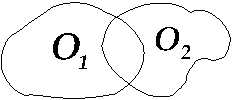
\includegraphics[width=2in]{CausalUnion.pdf}
\caption{The union of two domains}
\label{ }
\end{center}
\end{figure}
\par\noindent Note that this implies
\begin{equation}
\label{ }
\mathcal{O}_1\subset \mathcal{O}_2\ \implies\ \ \mathcal{A}(\mathcal{O}_1)\subset \mathcal{A}(\mathcal{O}_2)
\end{equation}
The local operators are obtained by taking the limit when a domain reduces to a point (this is not a precise or rigorous definition, in particular in view of the UV divergences of QFT and the renormalization problems).
\medskip\par\noindent
$\textdbend$ Caution, the observables of two disjoint domains are not independent if these domains are not causally independent (see below) since they can be related by dynamical/causal evolution.



\begin{figure}[h]
\begin{center}
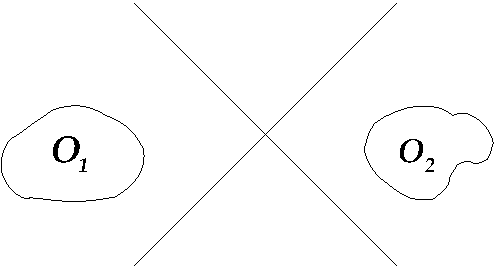
\includegraphics[width=3in]{CausalSeparated.pdf}
\caption{For two causally separated domains, the associated observables must commute}
\label{ }
\end{center}
\end{figure}


\paragraph{Causality:}
\index{Causality}
Secondly causality and locality must be respected, this implies that physical local observables which are causally independent must always commute. Indeed the result of measurements of causally independent observables is always independent of the order in which they are performed, independently of the state of the system.
Were this not the case, the observables would not be independent and through some measurement process information could be manipulated and transported at a faster than light pace.
If $\mathcal{O}_1$ and $\mathcal{O}_2$ are causally separated (i.e. any $x_1-x_2$, $x_1\in\mathcal{O}_1$, $x_2\in\mathcal{O}_2$ is space-like)) then  any pair of  operators $A_1$ and $A_2$ respectively in $\mathcal{A}(\mathcal{O}_1)$ and $\mathcal{A}(\mathcal{O}_2)$ commutes
\begin{equation}
\label{ }
\mathcal{O}_1\ \raisebox{1.ex}{$\bigvee$} \hskip -.77em \raisebox{-.8ex}{$ \bigwedge$}  \    \mathcal{O}_2\ ,\quad
A_1\in\mathcal{A}(\mathcal{O}_1) \ ,\quad
A_2\in\mathcal{A}(\mathcal{O}_2) \quad
\implies \quad
[A_1,A_2]=0
\end{equation}
This is the crucial requirement to enforce locality in the quantum theory.

\noindent{NB:} As already discussed, in theories with fermion, fermionic field operators like $\psi$ and $\bar\psi$ are not physical operators, since they intertwin different sectors (the bosonic and the fermionic one) and hence the anticommutation of fermionic operators does not contradict the above rule.


\paragraph{Causal completion:} 
\index{Causal completion}
One needs also to assume causal completion, i.e.
\begin{equation}
\label{ }
\mathcal{A}(\mathcal{O})=\mathcal{A}(\widehat{\mathcal{O}})
\end{equation}
where the domain $\widehat{\mathcal{O}}$ is the causal completion of the domain $\mathcal{O}$ ($\widehat{\mathcal{O}}$ is defined as the set of points $\mathcal{O}''$ which are causally separated from the points of $\mathcal{O}'$, the set of points causally separated from  the points of $\mathcal{O}$, see fig.\ref{f:CausComp} for a self explanating illustration).

\begin{figure}[h]
\begin{center}
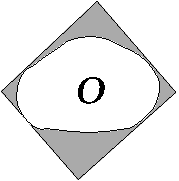
\includegraphics[width=1.5in]{CausalCompletion.pdf}
\caption{A domain $\mathcal{O}$ and its causal completion $\widehat{\mathcal{O}}$ (in gray)}
\label{f:CausComp}
\end{center}
\end{figure}

\par\noindent This implies in particular that  the whole algebra $\mathcal{A}$ is the (inductive) limit of the subalgebras generated by an increasing sequence of bounded domains whose union is the whole Minkovski space
\begin{equation}
\label{ }
\mathcal{O}_i\subset \mathcal{O}_j\ \text{if}\ i<j\ \text{and}\ \ \bigcup_i\mathcal{O}_i=\mathbb{M}^4\quad\implies\qquad \lim_{\longrightarrow}\mathcal{A}(\mathcal{O}_i)=\mathcal{A}
\end{equation}
and also that it is equal to the algebra associated to ``time slices'' with arbitrary small time width.
\begin{equation}
\label{ }
\mathcal{S}_\epsilon=\{\mathbf{x}=(t,\vec x):\ t_0<t<T_0+\epsilon\}
\end{equation}
\begin{figure}[h]
\begin{center}

\includegraphics[width=5in]{CausalSlice.pdf}
\caption{An arbitrary thin space-like slice of space-time is enough to generate the algebra of observables $\mathcal{A}$}
\label{f:CausalSlice}
\end{center}
\end{figure}

This indicates also why one should concentrate on von Neumann algebras.
The set of local subalgebras $\mathcal{L}= \{\mathcal{A}(\mathcal{O}):\ \mathcal{O}\ \text{subdomains of}\ M \}$ form an orthocomplemented lattice with interesting properties.

\paragraph{Poincar� invariance:}
\index{Poincar� invariance}
The Poincar� group $\mathfrak{P}(1,d-1)=\mathbb{R}^{1,d-1}\rtimes \mathrm{O}(1,d-1)$ must act on the space of local observables, so that it corresponds to a symmetry of the theory (the theory must be covariant under translations in space and time and Lorentz transformations).
When $\mathcal{A}$ is represented as an algebra of operators on a Hilbert space, the action is usually represented by unitary\footnote{Unitary with respect to the real algebra structure, i.e. unitary or antiunitary w.r.t. the complex algebra structure.} transformations $U(a,\Lambda)$ ($a$ being a translation and $\Lambda$ a Lorentz transformation).
This implies in particular that the algebra associated to the image of a domain by a Poincar� transformation is the image of the algebra under the action of the Poincar� transformation.
\begin{equation}
\label{ }
U(a,\Lambda)\mathcal{A}(\mathcal{O})U^{-1}(a,\Lambda)=\mathcal{A}(\Lambda\mathcal{O}+a)
\end{equation}
\begin{figure}[h]
\begin{center}
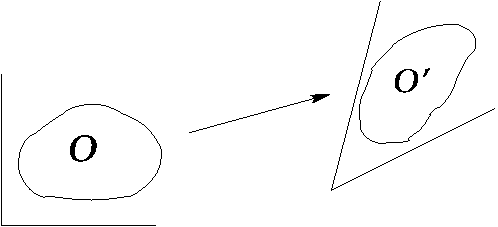
\includegraphics[width=3in]{CausalPoincare.pdf}
\caption{The Poincar� group acts on the domains and on the associated algebras}
\label{ }
\end{center}
\end{figure}

The generator of time translations will be the Hamiltonian $P_0=H$, and time translations acting on observables corresponds to the dynamical evolution of the system in the Heisenberg picture, in a given Lorentzian reference frame.


\paragraph{The vacuum state:}
\index{Vacuum}
Finally one needs to assume the existence (and the uniqueness, in the absence of spontaneous symmetry breaking) of a special state,  the vacuum state $|\Omega\rangle$. 
The vacuum state must be invariant under the action of the Poincar� transformations, i.e. 
$U(a,\Lambda)|\Omega\rangle = |\Omega\rangle$.
 At least in the vacuum sector, the spectrum of $\mathbf{P}=(E,\vec P)$ (the generators of time and space translations) must lie in the future cone.
 \begin{equation}
\label{ }
E^2-\vec p^2>0\quad,\qquad E>0
\end{equation}
 This is required since the dynamics of the quantum states must respect causality. In particular, the condition $E>0$ (positivity of the energy) implies that dynamical evolution is compatible with the modular automorphisms on the algebra of observables constructed by the Tomita-Takesaki theory.


\subsection{Axiomatic QFT}
\index{Axiomatic quantum field theory}

\subsubsection{Wightman axioms}
\index{Wightman axioms}

One approach to implement the program of algebraic  local quantum field theory is the so-called axiomatic field theory framework (Wightman \& G\aa rding).
Actually the axiomatic field theory program was started before the algebraic one.
In this formalism, besides the axioms of local, AQFT, the local operators are realized as ``local fields''. 
These local fields $\Phi$ are represented as distributions (over space-time $M$) whose values, when applied to some $C^\infty$ test function with compact support $f$ (typically inside some $\mathcal{O}$) are operators $\mathbf{a}=\langle \Phi{\cdot} f\rangle$.  Local fields are thus ``operator valued distributions''. 
\index{Local field}
They must satisfy the Wightman's axioms (see Streater and Wightman's book \cite{StreaterWightmanBook}  and R. Haag's book, again), which enforce causality, locality, Poincar� covariance, existence (and uniqueness) of the vacuum (and eventually in addition asymptotic completeness, i.e. existence of a scattering S-matrix).

\subsubsection{CPT and spin-statistics theorems}
\index{CPT theorem}
\index{Spin-statistics theorem}

The axiomatic framework is very important for the definition of quantum theories.
It is within this formalism that one can derive the general and fundamental properties of relativistic quantum theories
\begin{itemize}
  \item Reconstruction theorem: reconstruction of the Hilbert space of  states from the vacuum expectation values of product of local fields (the Wightman functions, or correlation functions),
  \item Derivation of the analyticity properties  of the correlation functions with respect to space-time $\mathbf{x}=(t,\vec x)$ and impulsion $\mathbf{p}=(E,\vec p)$ variables,
  \item Analyticity of the S matrix (an essential tool),
  \item The CPT theorem: locality, Lorentz invariance and unitarity imply CPT invariance,
  \item The spin statistics theorem,
  \item Definition of quantum field theories in Euclidean time (Osterwalder-Schrader axioms) and rigorous formulation of the mapping between Euclidean theories 
  and %$\leftrightarrow$
   Lorentzian quantum theories.
   \index{Euclidean space}\index{Minkowski space}
\end{itemize}

\section{Discussion}
I gave here a short introduction to the algebraic formulation of quantum mechanics and quantum field theory.
I did not aim at mathematical rigor nor completeness. 
I have not mentioned recent developments  and applications in the direction of gauge theories, of two dimensional conformal field theories, of quantum field theory in non trivial (but classical) gravitational background.

However I hope to have conveyed the idea that the ``canonical structure of quantum mechanics'' -- complex Hilbert space of states, algebra of operators, Born rule for probabilities -- is quite natural and is a representation of an underlying more abstract structure: a real algebra of observables  $+$ states, consistent with the physical concepts of causality, reversibility and locality/separability.


